\begin{figure}
\centering
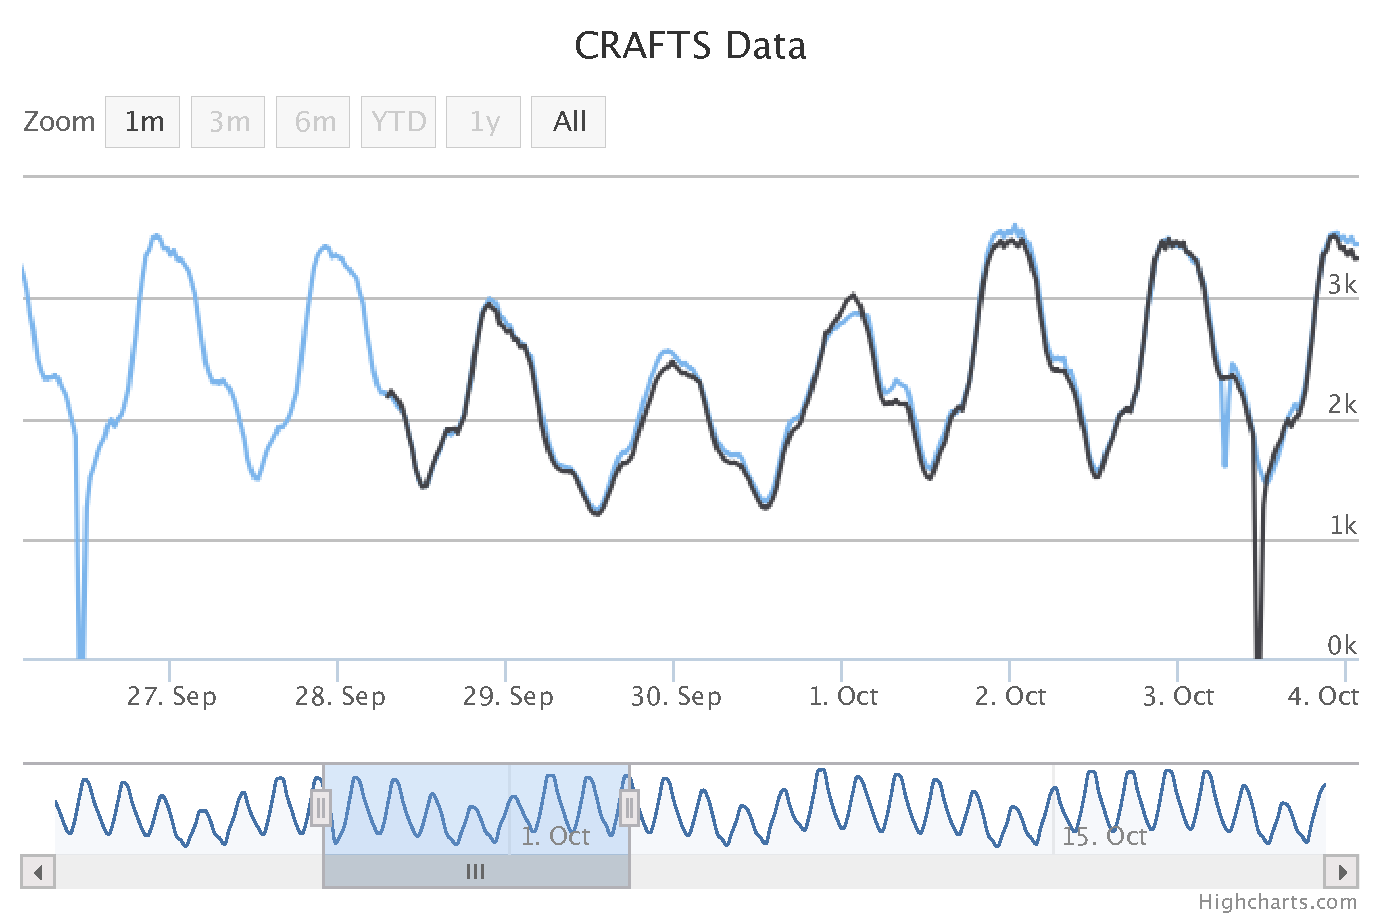
\includegraphics[width=\textwidth]{results/graphs/translation_outage.pdf}
\caption{An outage translated by the  predictor}
\label{fig:translation_outage}
\end{figure}

\begin{figure}
\centering
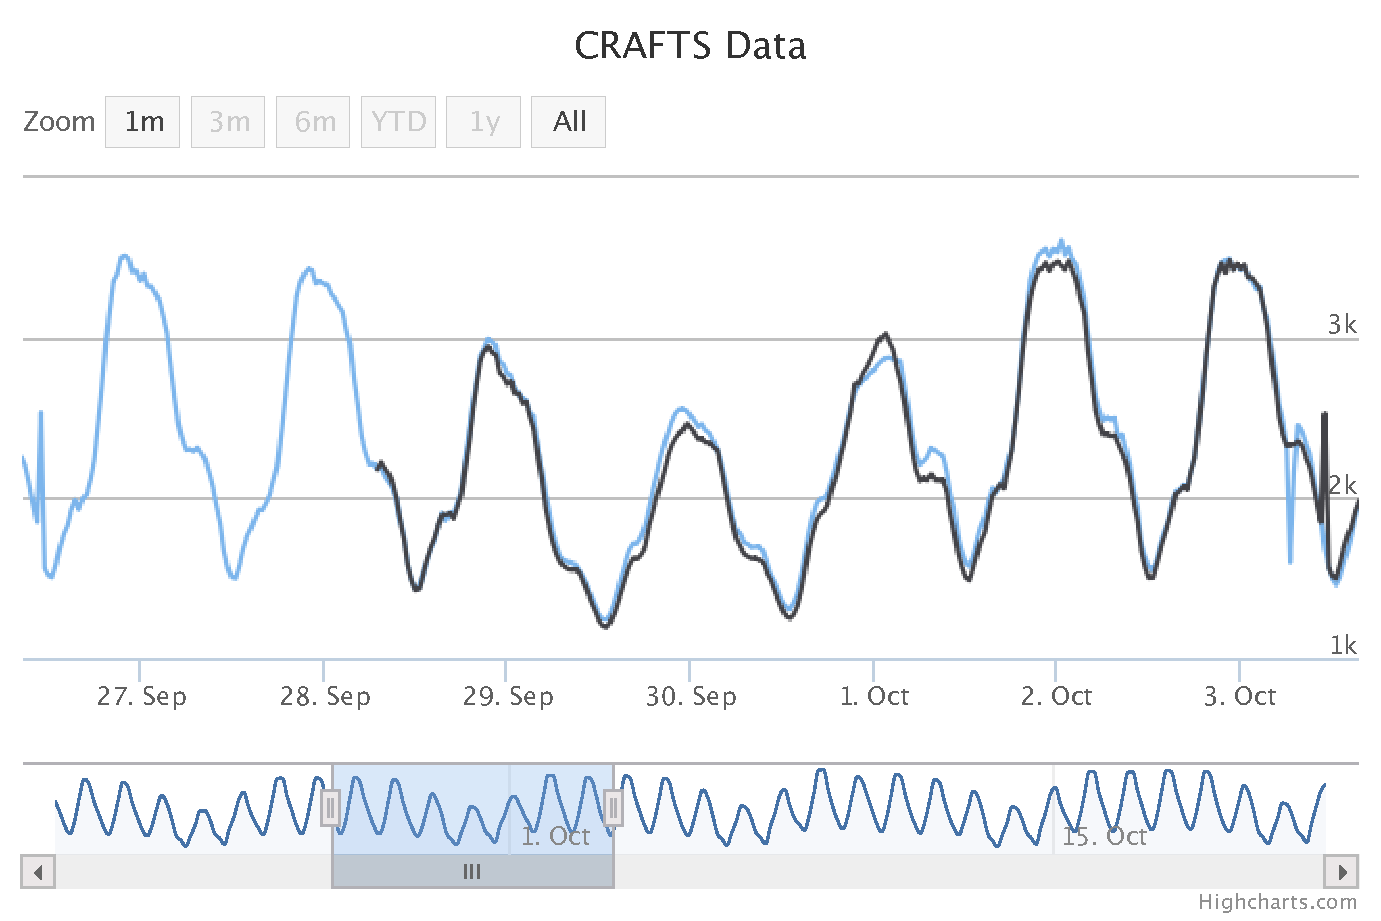
\includegraphics[width=\textwidth]{results/graphs/translation_spike.pdf}
\caption{A usage spike translated by the  predictor}
\label{fig:translation_spike}
\end{figure}

\begin{table}[H]
\centering
\begin{tabular}{| l | l | l |}
\hline
Type & RMSD & Percent \\ \hline
\end{tabular}
\caption{predictor results for the baseline workload}
\end{table}

% Outage workloads

\begin{table}[H]
\centering
\begin{tabular}{| l | l | l |}
\hline
Type & RMSD & Percent \\ \hline

\end{tabular}
\caption{predictor results for the 10-minute outage workload}
\end{table}

\begin{table}[H]
\centering
\begin{tabular}{| l | l | l |}
\hline
Type & RMSD & Percent \\ \hline

\end{tabular}
\caption{predictor results for the 30-minute outage workload}
\end{table}

\begin{table}[H]
\centering
\begin{tabular}{| l | l | l |}
\hline
Type & RMSD & Percent \\ \hline

\end{tabular}
\caption{predictor results for the 60-minute outage workload}
\end{table}

% Spike workloads

\begin{table}[H]
\centering
\begin{tabular}{| l | l | l |}
\hline
Type & RMSD & Percent \\ \hline

\end{tabular}
\caption{predictor results for the low spike workload}
\end{table}

\begin{table}[H]
\centering
\begin{tabular}{| l | l | l |}
\hline
Type & RMSD & Percent \\ \hline

\end{tabular}
\caption{predictor results for the mid spike workload}
\end{table}

\begin{table}[H]
\centering
\begin{tabular}{| l | l | l |}
\hline
Type & RMSD & Percent \\ \hline

\end{tabular}
\caption{predictor results for the high spike workload}
\end{table}